\newpage
\section{Main Memory}
Program must be brought (from disk) into memory and placed within a process for it to be run. 

Main memory, Register, Cache
\subsection{Background}
Memory Hierarchy

Memory Wall

Emerging NVM Technologies

Processing-in-Memory

\subsubsection{Base and Limit Registers}
\begin{figure}[!htb]
    \centering
    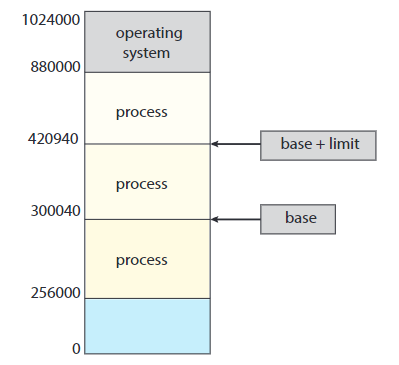
\includegraphics[width=0.309\textwidth]{pic/OS8/A base and a limit register define a logical address space}
    \caption{A base and a limit register define a logical address space}
\end{figure}

\subsubsection{Addresses Given in Different Ways}
\begin{itemize}
    \item Symbolic Address (such as the variable count)
    \item Relocatable Addresses (such as ``14 bytes from thebeginning of this module'').
    \item Absolute Addresses (such as 74014)
\end{itemize}


\subsubsection{Address Binding}
Address binding of instructions and data to memory addresses can happen at three different stages
\begin{itemize}
    \item Compile time: If memory location known a priori, absolute code can be generated
    \item Load time: Must generate relocatable code if memory location is not known at compile time
    \item Execution time: Binding delayed until run time 
\end{itemize}
\begin{figure}[!htb]
    \centering
    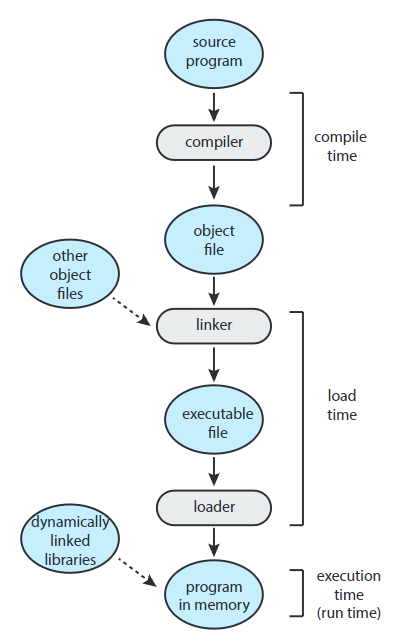
\includegraphics[width=0.22\textwidth]{pic/OS8/Multistep processing of a user program}
    \caption{Multistep processing of a user program}
\end{figure}

\subsubsection{Logical vs. Physical Address Space}
The concept of a logical address space that is bound to a separate physical address space is central to proper memory management
\begin{itemize}
    \item Logical address(CPU, also referred to as virtual address)
    \item Physical address
\end{itemize}
be the same in compile-time and load-time.\\
differ in execution-time

\begin{figure}[!htb]
    \centering
    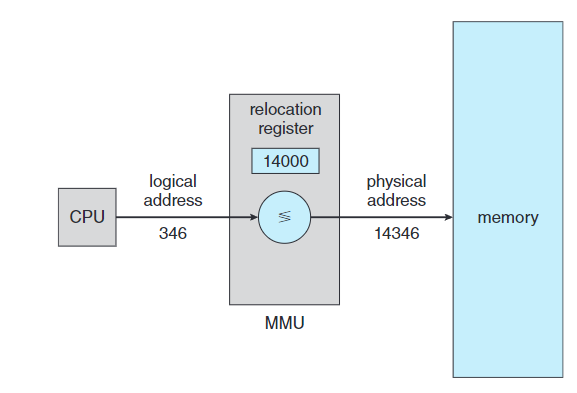
\includegraphics[width=0.309\textwidth]{pic/OS8/Dynamic relocation using a relocation register.}
    \caption{Dynamic relocation using a relocation register.}
\end{figure}
Memory-Management Unit (MMU): Hardware device that maps virtual to physical address

\subsubsection{Dynamic Loading}
Routine is not loaded until it is called

\subsubsection{Dynamic Linking}
Linking postponed until execution time. 
\begin{enumerate}
    \item Small piece of code, stub, used to locate the
    appropriate memory-resident library routine
    \item Stub replaces itself with the address of the routine,
    and executes the routine
\end{enumerate}
Dynamic linking is particularly useful for libraries. 


also known as shared libraries

\subsection{Contiguous Memory Allocation}
每个进程 自己的 view 实现物理内存的隔离. 

Main memory usually into two partitions:
\begin{enumerate}
    \item Resident operating system, usually held in low memory with
    interrupt vector
    \item User processes then held in high memory
\end{enumerate}

\subsubsection{Memory Protection}

\begin{figure}[!htb]
    \centering
    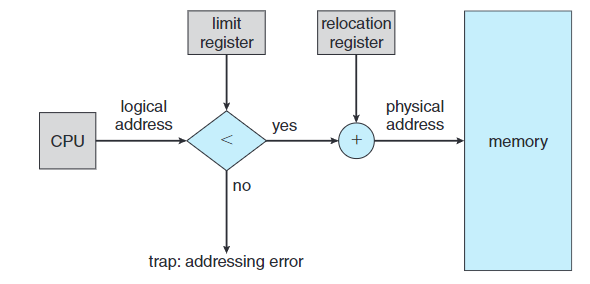
\includegraphics[width=0.42\textwidth]{pic/OS8/Hardware support for relocation and limit registers}
    \caption{Hardware support for relocation and limit registers}
\end{figure}
\begin{itemize}
    \item Relocation register contains value of smallest physical
    address
    \item Limit register contains range of logical addresses
\end{itemize}
MMU maps logical address dynamically


\subsubsection{Multiple-partition allocation}
When a process arrives, it is allocated memory from a hole large enough to accommodate it. 

Operating system maintains information about:
\begin{itemize}
    \item allocated partitions
    \item free partitions (hole)
\end{itemize}

Hole --- block of available memory; holes of various size are
scattered throughout memory

\begin{figure}[!htb]
    \centering
    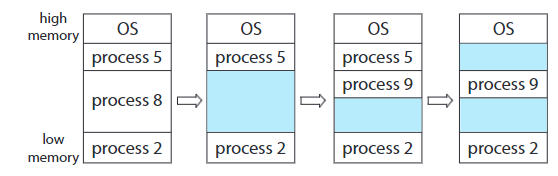
\includegraphics[width=0.42\textwidth]{pic/OS8/Variable partition}
    \caption{Variable partition}
\end{figure}

How to satisfy a request of size $n$ from a list of free holes:
\begin{itemize}\small
    \item First-fit: Allocate the first hole that is big enough
    \item Best-fit: Allocate the smallest hole that is big enough
    \item Worst-fit: Allocate the largest hole
\end{itemize}
First-fit and best-fit better than worst-fit in terms of speed and storage utilization

\subsubsection{Fragmentation}
\begin{itemize}
    \item External Fragmentation: total memory space exists to satisfy a
    request, but it is not contiguous
    \item Internal Fragmentation: allocated
    memory may be slightly larger than requested memory
\end{itemize}

Reduce external fragmentation by compaction. 但 move 的代价很大. 

\subsection{Paging}
Logical address space of a process can be noncontiguous;
process is allocated physical memory whenever the latter is
available
\begin{itemize}\small
    \item Divide physical memory into fixed-sized blocks called frames
    \item Divide logical memory into blocks of same size called pages
\end{itemize}
Internal fragmentation


\subsubsection{Address Translation Scheme}
Address generated by CPU is divided into:
\begin{itemize}
    \item Page number (p)
    \item Page offset (d) 
\end{itemize}

\begin{figure}[!htb]
    \centering
    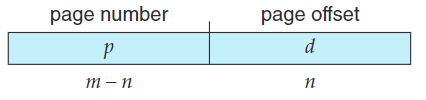
\includegraphics[width=0.309\textwidth]{pic/OS8/address }
    \caption{address}
\end{figure}


\begin{figure}[!htb]
    \centering
    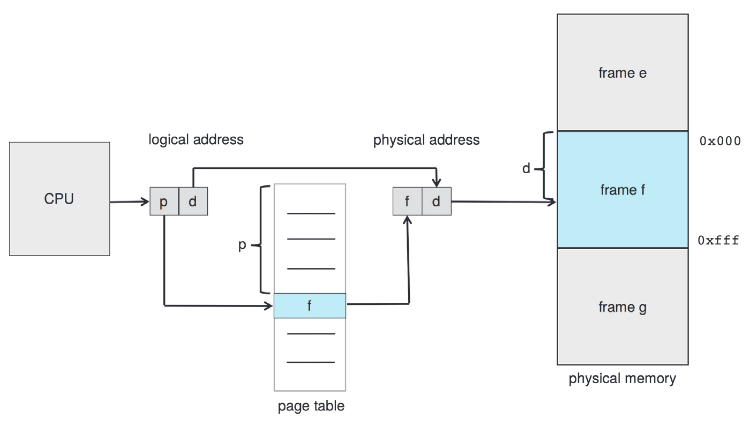
\includegraphics[width=0.42\textwidth]{pic/OS8/Paging hardware}
    \caption{Paging hardware}
\end{figure}

frame number (or called PPN)

\begin{figure}[!htb]
    \centering
    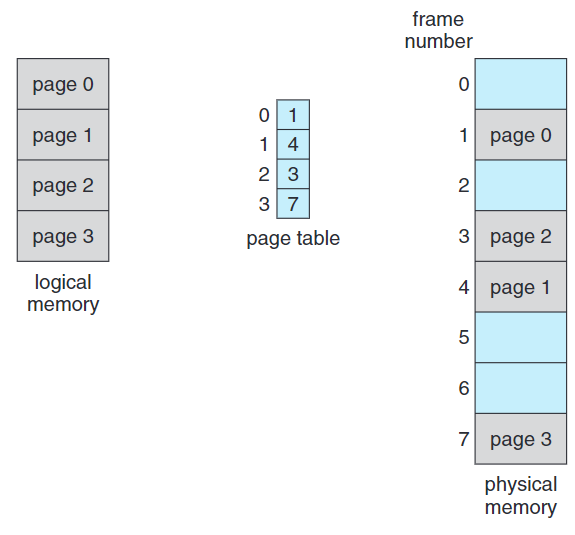
\includegraphics[width=0.309\textwidth]{pic/OS8/Paging model of logical and physical memory.}
    \caption{Paging model of logical and physical memory.}
\end{figure}

free-frame list 记录空闲的 frame. 

\subsubsection{Hardware Implementation of Page Table}
Page table is kept in main memory. 
\begin{itemize}\small
    \item Page-table base register (PTBR) points to the page table
    \item Page-table length register (PTLR) indicates size of the page table
\end{itemize}
这样每次访问 data/instruction 需要两次 memory, 一次 page table, 一次 data/instruction.

Solution: a special fast-lookup hardware cache called associative
memory or translation look-aside buffers (TLBs 转换旁视
缓冲, 一称快表)

Some TLBs store address-space identifiers (ASIDs) in
each TLB entry. (唯一标识每个进程,为该进程提供地址空间保护)

\begin{figure}[!htb]
    \centering
    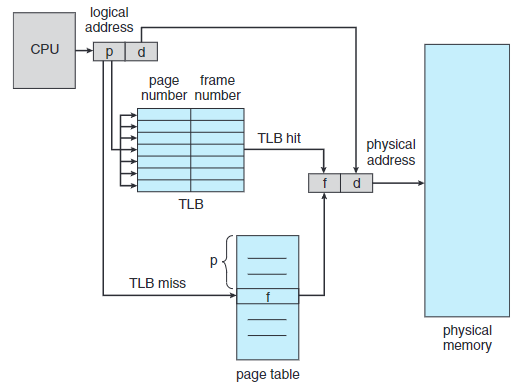
\includegraphics[width=0.4\textwidth]{pic/OS8/Paging hardware with TLB}
    \caption{Paging hardware with TLB}
\end{figure}

\subsubsection{Effective Access Time}
Associative Lookup $=\epsilon$ time unit. Assume memory cycle time is 1 microsecond. Hit ratio $=\alpha$

Effective Access Time (EAT):
\begin{align*}
    EAT &= (1+\epsilon)\alpha+(2+\epsilon)(1-\alpha)\\
    &=2+\epsilon -\alpha
\end{align*}

\subsubsection{Memory Protection in Paged Scheme}
Valid-invalid bit on PTE(page table entry). 访问 invalid 会产生 page fault. 

\begin{figure}[!htb]
    \centering
    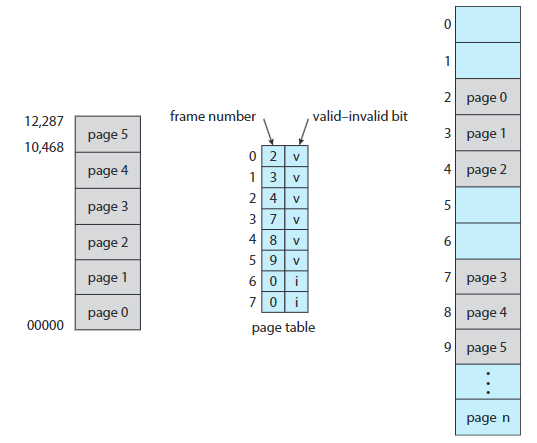
\includegraphics[width=0.309\textwidth]{pic/OS8/Valid (v) or invalid (i) bit in a page table.}
    \caption{Valid (v) or invalid (i) bit in a page table.}
\end{figure}

\subsubsection{Shared Pages}
\begin{itemize}
    \item Shared code 
    \item Private code and data
\end{itemize}

\begin{figure}[!htb]
    \centering
    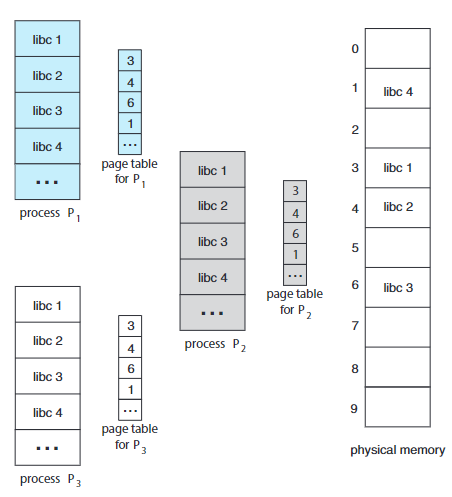
\includegraphics[width=0.309\textwidth]{pic/OS8/Sharing of standard C library in a paging environment}
    \caption{Sharing of standard C library in a paging environment}
\end{figure}


\subsection{Structure of the Page Table}
\subsubsection{Hierarchical Paging}
Break up the logical address space into multiple page tables --- to
page the page table

A simple technique is a two-level page table

\begin{figure}[!htb]
    \centering
    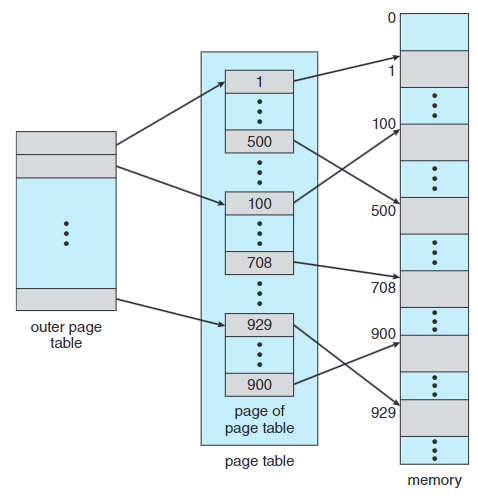
\includegraphics[width=0.309\textwidth]{pic/OS8/A two-level page-table scheme}
    \caption{A two-level page-table scheme}
\end{figure}

\paragraph{Two-Level Paging Example}A logical address (on 32-bit machine with 1K page size) is divided into:
\begin{itemize}
    \item a page number consisting of 52 bits
    \item a page offset consisting of 12 bits
\end{itemize}

Since the page table is paged, the page number is further divided into:
\begin{itemize}
    \item a 42-bit page number
    \item a 10-bit page offset
\end{itemize}

\begin{figure}[!htb]
    \centering
    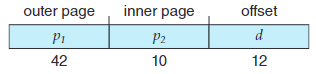
\includegraphics[width=0.22\textwidth]{pic/OS8/Two-Level Paging}
    \caption{Two-Level Paging}
\end{figure}

\begin{figure}[!htb]
    \centering
    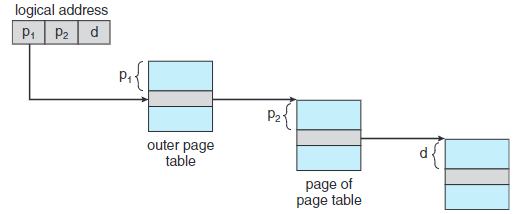
\includegraphics[width=0.42\textwidth]{pic/OS8/Address translation for a two-level 32-bit paging architecture}
    \caption{Address translation for a two-level 32-bit paging architecture}
\end{figure}

最多可能达到 7 级. 

在 linux 中: PGD $\to$ P4D $\to$ PUD $\to$ PMD $\to$ PTE

多级页表可以节省内存, 因为其空间是动态的. 


\subsubsection{Hashed Page Tables}
Common in address spaces $> 32$ bits. the clustered page table 处理 hash 冲突. 

\begin{figure}[!htb]
    \centering
    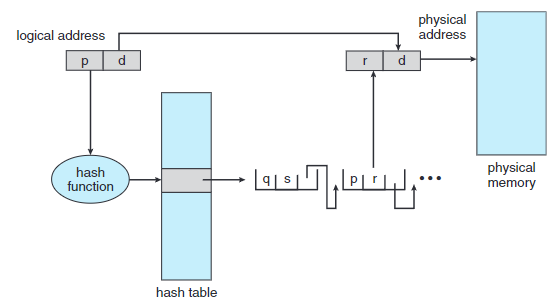
\includegraphics[width=0.42\textwidth]{pic/OS8/Hashed page table}
    \caption{Hashed page table}
\end{figure}

\subsubsection{Inverted Page Tables}
One entry for each real page of memory. 只有一个表, 相当于 memory 的微缩. 用物理的 i 查 p. 

\begin{figure}[!htb]
    \centering
    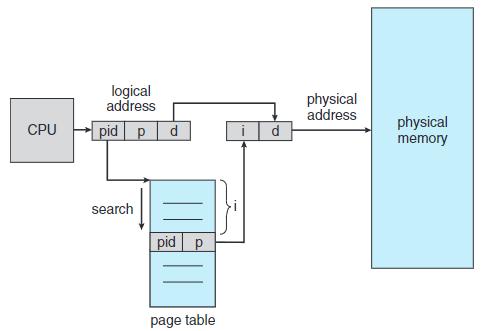
\includegraphics[width=0.309\textwidth]{pic/OS8/Inverted page table}
    \caption{Inverted page table}
\end{figure}
Search is slow, so put page table entries into a hash table. TLB can be used to speed up hash-table reference. 使用 content-addressible memory (CAM) 特殊硬件加速. 


\subsection{Swapping}
A process can be swapped temporarily out of memory to a backing store,
and then brought back into memory for continued execution. 

\begin{itemize}
    \item Backing store
    \item Roll out, roll in
\end{itemize}
System maintains a ready queue of ready-to-run processes which have
memory images on disk. 

只换一部分的 page, called page-in / page-out. 

\begin{figure}[!htb]
    \centering
    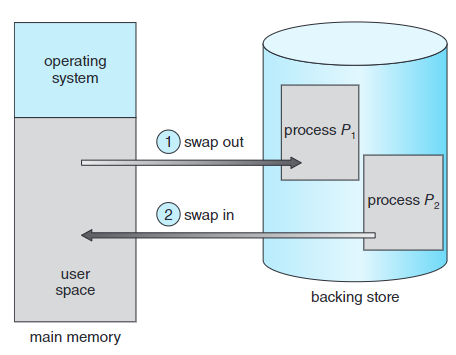
\includegraphics[width=0.309\textwidth]{pic/OS8/Standard swapping of two processes using a disk as a backing store}
    \caption{Standard swapping of two processes using a disk as a backing store}
\end{figure}

demand-paging 请求式调页. 

\subsection{Segmentation}
Memory-management scheme that supports user view of memory. 

A program is a collection of segments.

\begin{figure}[!htb]
    \centering
    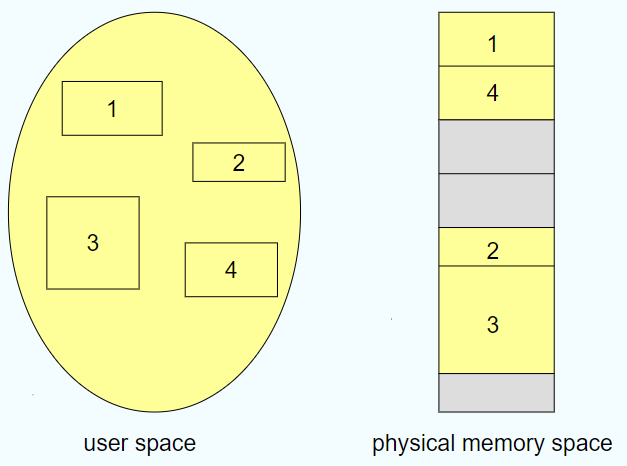
\includegraphics[width=0.309\textwidth]{pic/OS8/Logical View of Segmentation}
    \caption{Logical View of Segmentation}
\end{figure}

Logical address consists of a two tuple: \\
<segment-number, offset>,

Segment table --- maps two-dimensional physical addresses;
each table entry has:
\begin{itemize}
    \item base: contains the starting physical address where the
    segments reside in memory
    \item limit: specifies the length of the segment
\end{itemize}

\begin{itemize}\small
    \item Segment-table base register (STBR) points to the segment
    table's location in memory
    \item Segment-table length register (STLR) indicates number of
    segments used by a program
\end{itemize}

\begin{figure}[!htb]%FIXME 边框
    \centering
    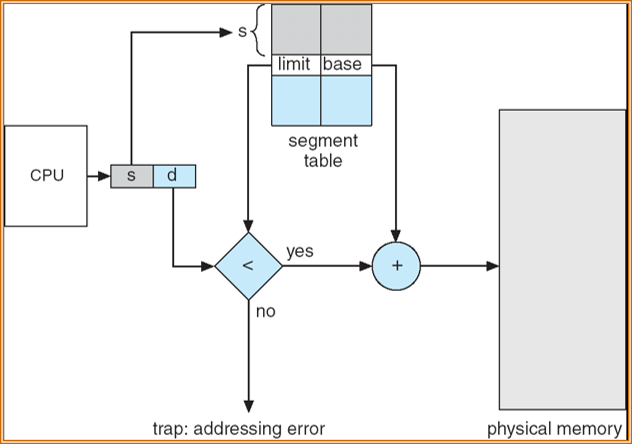
\includegraphics[width=0.309\textwidth]{pic/OS8/Segmentation Hardware}
    \caption{Segmentation Hardware}
\end{figure}
